\documentclass[11pt,a4paper]{article} % ein Artikel in 11-Punkt Schrift
% wie man sich schon denkt leitet % einen Kommentar bis Zeilenende ein

\usepackage[german]{babel} % deutsch, deutsche Rechtschreibung
\usepackage[utf8]{inputenc} % Unicode Text 
\usepackage[T1]{fontenc} % Umlaute und deutsches Trennen
\usepackage{mathptmx} % Times New Roman, gewohnter Font
\usepackage{courier} % Schreibmaschinenfont schicker
\usepackage[scaled=.95]{helvet} % was serifenloses wenn gebraucht
\usepackage{graphicx} % wir wollen Bilder einf��gen

\usepackage{listings} % Sch��ne Quellcode-Listings
\lstset{basicstyle=\sffamily, columns=[l]flexible, mathescape=true, 
  showstringspaces=false, numbers=left, numberstyle=\tiny}
\lstset{language=python} 
% und eine eigene Umgebung f��r Listings
\usepackage{float}
\newfloat{listing}{htbp}{scl}[section]
\floatname{listing}{Listing}

% Auch wenn es anr��chig ist, man kann den Platz etwas mehr ausn��tzen
\usepackage[paper=a4paper,width=14cm,left=35mm,height=22cm]{geometry}
\usepackage{setspace}
\linespread{1.10} % nicht ganz anderthalbzeilig, nur ein bisschen mehr Platz
\setlength{\parskip}{0.5em} % kleiner Paragraphenabstand
\setlength{\parindent}{0em} % im Deutschen Einr��ckung nicht ��blich, leider

% Seitenmarkierungen 
\usepackage{fancyhdr} % Schickere Header und Footer
\pagestyle{fancy}
% font f��r Header/Footer
\newcommand{\phv}{\fontfamily{phv}\fontseries{m}\fontsize{9}{11}\selectfont}
\fancyhead[L]{\phv Praktikumsbericht} 
\fancyhead[R]{\phv \thepage}
\fancyfoot[L]{\phv Aoe GmbH}
\fancyfoot[C]{\ } % keine Seitenzahl unten
\fancyfoot[R]{\phv Michael Sandritter}

% Ein spezielles Paket zum Aufteilen des Literaturverzeichnisses
\usepackage{bibtopic}
\makeatletter
\def\@seccntformat#1{%
  \expandafter\ifx\csname c@#1\endcsname\c@section\else
  \csname the#1\endcsname\quad
  \fi}
\makeatother

\title{Praktikumsbericht}
\author{Michael Sandritter \\ AOE GmbH}

\date{\today}

\begin{document}
\maketitle % erzeugt den Titel mit Autor und Datum


\newpage % neue Seite, muss bei einem Artikel eigentlich nicht sein

\section{Praktikumsbetrieb} \label{sec:betrieb} 
% mit \label k��nnen wir die Einf��hrung referenzieren

Mein Praktikum habe ich bei der AOE GmbH in Wiesbaden absolviert. 
Die AOE GmbH hat seinen Hauptsitz in Wiesbaden und ist Dienstleister für Open
Source Enterprise Lösungen.
AOE wurde 1999 unter dem Firmennamen AOE media gegründet und arbeitete
anfänglich als TYPO3 Dienstleister.
Inzwischen umfassen die Serviceleistungen Open Source Web Portale, E-Commerce und mobile Anwendungen, 
die für globale agierende Unternehmen entwickelt werden. 
Das Kollegium umfasst 180 Entwickler und Consultants an 8 Standorten, davon 120 Mitarbeiter in der Zentrale in Wiesbaden. 
Die Unternehmenskultur setzt auf die Kernelemente: Open Source, objektorientierte Programmierung und Methoden 
wie Agile Software-Entwicklung und Test-Driven-Development. 

Dabei pflegt die AOE GmbH eine dezentrale Unternehmensstruktur. Jedem Kunden wird ein Team aus Entwicklern zur Seite gestellt. 
Das Team arbeitet von dort ab komplett selbstständig und setzt alle
Projektphasen in engem Kontakt mit dem Kunden um.

\section{Arbeitsumfeld} \label{sec:umfeld}

In meinem Praktikum wurde ich vorwiegend als Backend-Entwickler im Congstar-Team eingesetzt. 
Das Team bestand dabei aus 19 Entwicklern und acht Testern, die sich ihrerseits wieder in 3 kleinere Teams aufteilen.  
Die Frontend bzw. Backend-Kompetenzen waren dabei gleichmäßig auf die 
verschiedenen Teams verteilt, so dass jedes Team, für sich, in der Lage war sowohl Backend- als auch
 Frontend-Tasks zu übernehmen.

Jedes Team arbeitet nach der agilen Softwareentwicklungsmethodik Scrum. 
In täglichen Daily Meetings tauschen sich die Entwickler in ihren kleinen Teams
über den aktuellen Entwicklungsstand aus, indem jeder Entwickler und Tester, dem
Team erzählt, woran er gerade arbeitet und gegebenenfalls schildert welche
Probleme bei der Umsetzung existieren.
Zusätzlich finden zwei mal wöchentlich Weekly Meetings statt, 
bei denen alle Entwickler und Tester zu einem übergreifenden Update des
Entwicklungsstand zusammenkommen.
In der großen Runde werden Themen besprochen, die das komplette Team betreffen. 
Dazu gehört zum Beispiel, das Einführen und Verwenden neuer Technologien, das
Entwickeln oder ändern der Software Architektur und generelle organisatorische
Themen.

Der zeitliche Rahmen gibt vor, dass dem Kunden alle zwei Monate ein neues Softwarepaket mit neuen Features ausgeliefert wird. 
Innerhalb dieser Zeit absolviert, jedes Team drei Sprints. Die ersten beiden Sprints sind Feature Sprints, 
die jeweils 3 Wochen Arbeitszeit umfassen. In diesen beiden Sprints werden neue Stories umgesetzt, 
die davor von den Product Ownern (PO) priorisiert worden sind. Das Team
entscheidet jedoch für jeden Sprint neu, wie viele Stories realistisch umsetzbar sind und arbeitet zu jeder Story kleinere Tasks aus, 
die von den Entwicklern geclaimed und umgesetzt werden. Der letzte
Sprint innerhalb der zwei Monate ist ein Release Sprint.
Dieser erstreckt sich über die beiden verbleibenden Wochen. 
Zu dieser Zeit finden Verbundtests statt, bei denen die neu entwickelten Features im Zusammenspiel mit der $Aax^{2}$ getestet wird. 

Die $Aax^{2}$ ist die Software aus dem Hause Compax. Diese hält dencongstar-spezifischen Produktkatalog.
Darin werden alle Congstar Produkte abgebildet, wie zum Beispiel die Post- und
Prepaidtarife, mit den dazugehörigen Buchungsoptionen.
Die $Aax^{2}$ bietet dafür Soap-Schnittstellen an, um die Produktdaten im, von
AOE entwickelten, Backend beziehen zu können.

Infolge des Release Sprints, besteht für die Entwickler ein Entwicklungs-Stop, 
so dass das neue Softwarepaket im Verbundtest getestet werden kann. Anstatt an neuen Features weiter zu arbeiten, 
wird die Zeit einerseits zum refactorn der Software und zum anderen zum update von Frameworks und anderer Software genutzt.

Am Ende jedes Sprints findet zusammen mit den Stakeholdern das Review statt, 
bei dem das Entwickler-Team die Ergebnisse des aktuell endenden Sprints
präsentieren.
Dafür fahren die Entwickler-Teams nach jedem Feature-Sprint nach Köln zu
Congstar, während sich die Beteiligten nach Ende des Release-Sprints bei Aoe in
Wiesbaden treffen.
Hauptsächlich geht es um die Präsentation der Stories, die innerhalb des
Sprints erfolgreich umgesetzt werden konnten.
Das Entwickler-Team berichtet in diesem Zusammenhang was während des Sprints gut
gelaufen ist, welche technischen Probleme und Hindernisse sich ergeben haben und
wie diese Probleme gelöst wurden. Die Stakeholder haben in diesem Zuge die
Möglichkeit offene Fragen mit den Entwicklern direkt zu klären. Alle Beteiligten
erhalten somit einen Überblick über den aktuellen Stand des Projekts, der sich
im Produkt-Backlog widerspiegelt.
Das Review dient somit als Grundlage für das darauf folgende Sprint Planning.

Im Sprint Planning wird im ersten Teil besprochen, welche Stories und wie viele Stories 
im Laufe des nächsten Sprints umgesetzt werden können. Während im zweiten Teil
besprochen wird, wie diese Stories umgesetzt werden sollen.
Dies geschieht im Zusammenspiel von Entwickler-Team, PO und Scrum Master. Gemeinsam priorisieren sie das Sprintziel. 
Dafür werden die Stories im Backlog priorisiert und für jede Story eine
Aufwandsschätzung durch die Entwickler abgegeben.
Parallel wird grob berechnet wie groß die Velocity des Teams ist, um
einordnen zu können wie viele Stories innerhalb eines Sprints tatsächlich
umgesetzt werden können. Nachdem die Stories für den nächsten Sprint
festgelegt sind, definieren die Entwickler für jede Story kleinere Tasks.

Backlog, Stories und Tasks werden im Projekt-Management-Tool
zugänglich gemacht. Aktuell wird als solches Tool Kunagi verwendet. Künftig
soll Kunagi jedoch durch JIRA ersetzt werden.

Im Laufe des Sprints werden die einzelnen Tasks von den Entwicklern abgearbeitet.
Diese müssen dabei vermerken, wie viel Zeit sie für den Task geburned, sprich benötigt haben. Aus der
geschätzen und der letztendlich benötigten Zeit lässt sich ein Burndown-Chart
ermitteln, das den aktuellen Fortschritt des Sprints widerspiegelt.

Sind alle Tasks einer Story umgesetzt steht die Abnahme dieser Story an. Diese erfolgt 
durch einen Entwickler der an der Umsetzung der Story beteiligt war und durch den Product Owner. 
Der Entwickler präsentiert dem PO die Features, die durch die Story umgesetzt
werden sollten.
Erfüllt das Umgesetzte alle Akzeptanz-Kriterien, die für die Story definiert
wurden, kann die Story durch den PO abgenommen werden und ist fertig.

\section{Projektbeschreibung} \label{sec:projekt}

Entwickelt wird der Webshop der Firma Congstar. Congstar ist als Schwestergesellschaft der Telekom, 
deutschlandweiter Anbieter für Mobilfunk- und DSL-Produkte. 

Dem Kunden soll zum einen abhängig von seinem Endgerät alle relevanten
Informationen zum Congstar Portfolio und Service dargestellt bekommen und
unabhängig von seinem Endgerät, neue Verträge abschließen und bestehende
Verträge verwalten können.

Für die Redakteure von Congstar sollen spezielle Informationen des Webshops
redaktionell und zentral pflegbar sein, um inhaltliche Inkonsistenzen und redundante Informationen zu vermeiden. 

\section{Deployment Pipeline} \label{sec:pipeline}

Im folgenden wird der Ablauf der Deployment-Pipeline erläutert. 
\begin{figure}[h]
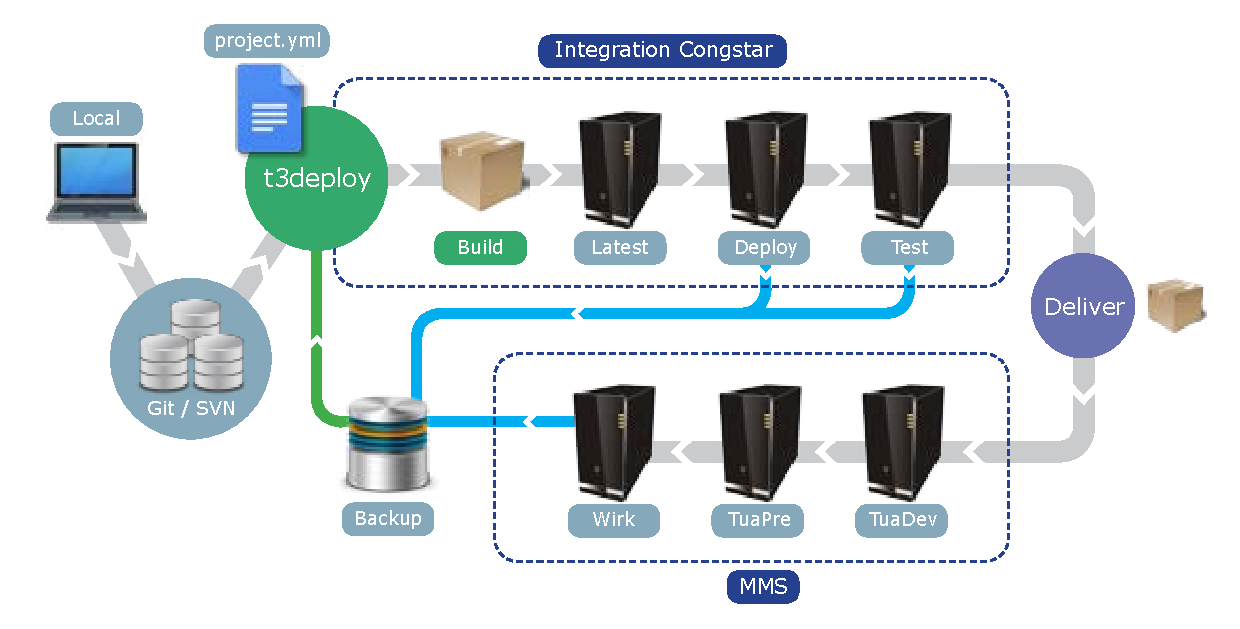
\includegraphics[width=\textwidth]{images/DeploymentPipeline.pdf}
\centering
\end{figure}
 
Der grobe Ablauf des Deployments sieht so aus, dass ein aktuelles Backup aller System, auf denen relevante Daten gepflegt werden müssen, erstellt und in das Backupstorage geschrieben werden. Dabei werden die Systeme vor einem Deployment gesperrt um zu verhindern, dass die Daten nach dem Backup noch verändert werden. 


Die verschiedenen Systeme verteilen sich auf zwei Hosts:

\begin{itemize}
  \item Integration Congstar
  \item MMS (T-Systems Multimedia Solution)
\end{itemize}

Wird ein Softwarepaket komplett neu gebaut, wird zum einen der Quellcode aus den getagten Git-Repositories gezogen und zum anderen die Datenbank und andere Bewegungsdateien aus dem Backupstorage (jeweils von den relevanten Systemen) zusammengeführt. 

Die Verheiratung findet mit der Deploymentsoftware T3deploy statt. Mit Hilfe der Konfigurationsdatei project.yml baut die T3Deploy Software ein fertiges, installierbares Softwarepaket. Die Konfigurationsdatei 
enthält dabei alle Infos über Extensions, Libraries und Datenbanken, die zum Bau eines Pakets notwendig sind.

War der Bau eines Pakets erfolgreich, wird dieses zur erst auf den aoe-internen Umgebungen des Integration Congstar installiert und durchläuft mehrere Teststufen.

Auf der Latest Umgebung werden alle automatisierten Tests durchgeführt. Dazu gehören Unit-Tests, Smoke Tests, sämtliche Code Metriken und Static Cache Tests. Laufen dort alle Tests durch kann das Paket auf der Deploy Umgebung installiert werden. Dort haben die Redakteure von Congstar die Möglichkeit redaktionelle Änderungen vorzunehmen. Zusätzlich werden auf dieser Umgebung neue Nutzer für das Typo3-Backend angelegt, die über das Backupstorage in jedem gebauten Paket zugänglich gemacht werden. Die letzte Umgebung des Integration Congstar bildet die Test Umgebung. Dort laufen hauptsächlich Java Sellenium Tests.

Sind alle drei aoe-internen Teststufen durchlaufen wird einmal täglich nachts ein fertiges Paket an die MMS geliefert und dort auf der TuADev (Test und Abnahme) Umgebung installiert. Auf der TuADev Umgebung werden Abnahmetests seitens Congstar Testern durchgeführt, die hauptsächlich Sellenium Tests umfassen.

//TODO über die TuAPre und Wirk Umgebung schreiben. 


\section{Feature 01: Extension zur Reisekostenkalkulation} \label{sec:pipeline}

Da viele Softwaremodule des Congstar Webshops also Typo3 Extensions umgesetzt sind, habe ich im Zuge 
meiner Einarbeitung eine eigene Extension entwickelt, die als Reiseplanungstool eingesetzt werden kann.
Ziel der Extension ist es, Personen eine grobe Kalkulation der Kosten offenzulegen, über Reiseziele, die sie gerne bereisen würden, von denen sie aber nicht wissen, welche Kosten auf sie zukommen. 





\newpage

% Listen, wenn ��berhaupt!, bitte ans Ende und nicht an den Anfang
%\listoffigures % Liste der Abbildungen 
%\listoftables % Liste der Tabellen

\newpage

% Als letztes noch das Literaturverzeichnis
\bibliographystyle{plain}
% so w��re es ganz einfach!
%\bibliography{ausarb,online}
% dann mit "bibtex ausarb" bibtexen und das Literaturverzeichnis ist da

% z.B. mit bibtopic kann man die Quellen sauber trennen
\begin{btSect}{ausarb}
\section*{Literaturverzeichnis}
\btPrintCited
\end{btSect}
\begin{btSect}{online}
\section*{Online-Quellen}
\btPrintCited
\end{btSect}
% dann mit "bibtex ausarb1" und "bibtex ausarb2" arbeiten
% Wir verwenden ausarb<i> weil die Dokumenten-Datei ausarb.tex ist

\end{document}
